\section{Das Potential-Problem}\label{kap_pot}

Im Folgenden werde ich das Hauptthema dieser Bachelorarbeit, das Potential-Problem, beschreiben und erklären.

\begin{mydef}\label{def_potential}
	Das Potential $k$ ist eine Art Kontostand, mit dem eine oder mehrere Kantengewichte reduziert werden können. Die Größe des Potentials gibt an, um wie viel die Gewichte insgesamt reduziert werden dürfen. 
\end{mydef}
Durch die Anwendung des Potentials soll sich die Anzahl der benötigten Agenten möglichst stark reduzieren. Diese Agentenzahl ändert sich unterschiedlich stark oder auch gar nicht, je nachdem, auf welche Kanten das Potential angewendet wird. Der Algorithmus soll daher das Potential optimal nutzen, um die Agentenzahl möglichst stark zu senken, indem die Kante(n), die für die hohe Agentenzahl verantwortlich sind, reduziert werden.
\\
\\
Wir werden verschiedene Varianten des Potential-Problems betrachten und für jede Variante einen Algorithmus angeben, sowie kurz Laufzeit und Korrektheit begründen.

\subsection{Spezialfall $k = 1$}\label{kap_pot=1}

Zunächst wird das Potential-Problem $k = 1$ beschrieben, da dies die einfachste Variante ist. In dieser Variante darf auf genau einer beliebigen Kante das Kantengewicht um genau 1 reduziert werden. Allerdings muss das Gewicht der Kante nach der Reduzierung weiterhin $\omega \geq 1$ sein. Ziel ist es, das Potential so anzuwenden, dass die Anzahl der Agenten möglichst gut gesenkt wird.


\subsubsection{Algorithmusidee}

Jeder Knoten berechnet im Algorithmus von \cite{cima_paper} die minimale Anzahl von Agenten (siehe Kapitel \ref{modifizierterAlgoChapter}), und es wird schnell klar, dass die Höhe der Agentenanzahl an jedem Knoten von bestimmten Kanten mit ihren Gewichten abhängen muss.
\\
\\
Die Idee, um das Potential-Problem für den Spezialfall $k = 1$ zu lösen, ist nun, die Abhängigkeiten zu speichern, welche Kanten die Agentenzahl in jedem Knoten beeinflussen. Dazu wird im modifizierten Algorithmus (aus Kapitel \ref{modifizierterAlgoChapter}) protokolliert, wie jede berechnete Nachricht zustande kommt, also von welchen Kanten sie abhängt.
\\
\\ 
Wie im Algorithmus beschrieben, kann man sehen, dass eine Nachricht $\lambda_{y}$ aus drei verschiedenen Fällen entstehen kann:

\begin{enumerate}[label=\alph*)]
	
	\item aus den beiden größten Kanten $\lambda_{y} \gets edge_{1} + edge_{2}$ \label{entstehung_nachricht_max1+max2}
	
	\item aus der Kante, über welche die Nachricht gerade verschickt wird (diese entspricht dem Knotengewicht) $\lambda_{y} \gets \omega(x)$
	
	\item aus der größten angekommenen Nachricht $\lambda_{y} \gets l_{1}$

\end{enumerate}

Je nachdem, durch welchen Fall eine Nachricht $\lambda_{y}$ berechnet wird, kommen andere Kanten in Frage, die protokolliert werden müssen.
Allerdings gilt für alle Fälle, dass sich der Algorithmus maximal zwei Kanten merken muss, da ansonsten die minimale Agentenzahl nicht verringert werden kann. Gibt es keine oder mehr als zwei Kanten, so wird protokolliert, dass das Potential an dieser Stelle nicht eingesetzt werden kann, um die Agentenzahl zu reduzieren (es wird eine "`flag"' gesetzt).

\begin{theorem}\label{theorem_max2kanten}
	Es müssen maximal zwei Kanten pro Nachricht protokolliert werden. Ansonsten kann das Potential nicht angewendet werden.
\end{theorem}

\begin{proof}
	Wir beweisen dieses Theorem, indem wir einen Widerspruch erzeugen. Wir nehmen an, es könnten mehr als zwei Kanten pro Nachricht protokolliert werden, o.B.d.A. seien es drei Kanten. Dies würde bedeuten, dass durch Reduzierung einer dieser drei Kanten die Nachricht verkleinert werden könnten. Die Berechnung der Nachricht pro Fall hängt aber nur von maximal zwei Kanten ab (bei dem gerade beschriebenen Fall \ref{entstehung_nachricht_max1+max2} $\lambda_{y} \gets edge_{1} + edge_{2}$). Dies bedeutet, dass die drei Kanten aus zwei verschiedenen Fällen stammen müssen. Wenn also nun eine der drei Kanten reduziert wird, kann sich maximal nur ein Fall verkleinern, der andere bleibt unverändert. Da der Fall ausschlaggebend ist, der die größte Nachricht generiert, wird durch die Reduzierung der Kante die Nachricht nicht verändert, da der nicht veränderte Fall immer noch die alte Nachricht generiert. Da aber gesagt wurde, dass alle drei Kanten die Nachricht reduzieren können, ist dies ein Widerspruch dazu, dass eine Nachricht von mehr als zwei Nachrichten abhängen kann.
\end{proof}

\subsubsection{Die Protokollierung in der Nachricht}

Im Folgenden wird bei allen drei möglichen Fällen beschrieben, welche Kanten unter welcher Bedingung protokolliert werden. Um dies protokollieren zu können, wird die Nachricht etwas erweitert. Sie enthält nun nicht mehr nur die Anzahl der Agenten, die für den Teilbaum benötigt werden, sondern auch die (bis zu) zwei protokollierten Kanten bzw. einen "`flag"', falls keine eindeutigen Kanten bestimmt werden konnten. Die Berechnung der Nachricht bleibt unverändert. Es wird nur zusätzlich folgende Protokollierung in den drei Fällen eingeführt: 

\begin{enumerate}[label=\alph*)]
	
	\item In diesem Fall wird die Nachricht aus den beiden größten Kanten berechnet ($\lambda_{y} \gets edge_{1} + edge_{2}$). Allerdings muss kontrolliert werden, ob diese zwei Kanten eindeutig sind, oder ob es evtl. mehrere gleich große Kanten gibt. Ist die Wahl der Kanten nicht eindeutig, muss dies bei der Protokollierung mit berücksichtigt werden. Es gilt $edge_{1} \geq edge_{2} \geq edge_{3}$:

		\begin{algorithmic}
			\If {$edge_{1} == edge_{3}$}
			\LineComment{Es gibt (mindestens) drei gleich große Kanten. Selbst wenn man eine der drei Kanten reduziert, wird die Nachricht aus den anderen beiden Kanten berechnet und dadurch nicht verkleinert.}
			\State \uline{protokolliere: "`flag"'}
			\ElsIf {$edge_{2} == edge_{3}$}
			\LineComment{Die maximale Kante ist eindeutig, die zweit größte Kante nicht. Es macht daher nur Sinn die größte Kante zu reduzieren.}
			\State \uline{protokolliere: $edge_{1}$}
			\Else
			\LineComment{Sowohl die größte als auch die zweit größte Kante ist eindeutig. Wir können eine von den beiden reduzieren, um auch die Nachricht erfolgreich zu verkleinern.}
			\State \uline{protokolliere: $edge_{1}$ und $edge_{2}$}
			\EndIf
		\end{algorithmic}
		
	\clearpage
		
	
	\item Die Nachricht ist kleiner als das Knotengewicht: $\omega(x) > edge_{1}+edge_{2}$. Da aber $\omega(x)$ so definiert ist, dass es den Wert des größten Kantengewichts inzident zu $x$ hat, muss die Kante ausschlaggebend sein, über die die Nachricht verschickt wird. 
	\\
	Diese Kante $e = \{x, y\}$ zwischen $x$ und $y$ ist für den Nachrichtenwert also entscheidend und wird somit in der Nachricht protokolliert: \uline{Protokolliere: $e = \{x, y\}$}
	
	\item In diesem Fall bestimmt die größte ankommende Nachricht $l_{1}$ die neu berechnete Nachricht. Da keine weitere Kante mehr Einfluss genommen hat, werden die protokollierten Kanten (oder die "`flag"') aus $l_{1}$ für $\lambda_{y}$ übernommen: \uline{Protokolliere: das gleiche wie $l_{1}$}
	
\end{enumerate}
Wichtig ist noch zu beachten, dass mehrere Fälle gleichzeitig auftreten können. Passiert dies, muss man einen weiteren Test durchführen, ob die verschiedenen Fälle unterschiedliche Kanten bzw. "`flag"' protokollieren würden.
\\
Würden die Fälle verschieden protokollieren, so protokolliere "`flag"', da es keine eindeutige(n) Kante(n) gibt. Das Potential kann an dieser Stelle nicht genutzt werden. Würden die verschiedenen Fälle exakt die gleiche(n) Kante(n) protokollieren, so wird diese Protokollierung für $\lambda_{y}$ übernommen.
\\
\\
Außerdem macht es nur Sinn, Kanten zu protokollieren, welche ein Kantengewicht $\omega > 1$ haben, da diese Kante ansonsten nicht durch das Potential reduziert werden kann. Es macht aber kein Sinn, Kanten zu protokollieren, welche nicht reduziert werden können. Diese Überprüfung muss bei jeder Kante durchgeführt werden, die protokolliert werden soll.

\subsubsection{Protokollierung im Knoten}

Die Berechnung der $\mu$ an jedem Knoten funktioniert analog zur Nachrichtenberechnung. Auch in den Knoten wird gespeichert, von welchen Kanten der Wert abhängt. Dies ist entweder $edge_{1}$ und $edge_{2}$, oder die Kanten, die in $l_{1}$ protokolliert sind.
\\
\\
Nachdem jeder Knoten $x$ den Wert $\mu(x)$ berechnet und die Kanten gespeichert hat, von denen dieser Wert abhängt, geht der Algorithmus durch alle Knoten durch und speichert von jedem Knoten $i$, für den gilt $\mu(i) = \mu(h)$ - wobei $h$ die Homebase ist - von welchen Kanten dieser Knoten $i$ abhängt, in einer Liste $L$. \\
Das Potential wird auf eine dieser in $L$ gespeicherten Kanten angewendet, um die Anzahl der Agenten zu minimieren. Alle Kanten, die in $L$ gespeichert sind, verringern die Anzahl an Agenten, da sie von einem Knoten mit minimaler Agentenzahl protokolliert wurden, und somit diesen Knoten um genau 1 reduzieren. Falls das Potential $k = 1$ nicht angewendet werden kann, ist $L$ leer.

\subsubsection{Laufzeit und Korrektheit}


	\begin{theorem}
		Die Protokollierung, und somit die Berechnung der Kante, auf die das Potential $k=1$ angewendet werden sollte, ist in linearer Laufzeit möglich.
	\end{theorem}
	\begin{proof}
		Um die Laufzeit abzuschätzen, reicht es, die Berechnung der Nachrichten zu betrachten, da nur diese für den Algorithmus verändert wurde. Die Anzahl der zu berechnenden Nachrichten weicht nicht von der benötigten Anzahl des Algorithmus in Kapitel \ref{modifizierterAlgoChapter} ab. Außerdem kann die Protokollierung für jede Kante in konstanter Zeit durchgeführt werden. Für jede Nachrichtenberechnung muss nur eine einfache Fallunterscheidung durchgeführt werden, um zu ermitteln, welche Kante in der aktuellen Nachricht protokolliert werden muss. Da es $O(n)$ viele Nachrichten gibt, die alle in $O(1)$ berechnet werden können, bleibt die Laufzeit, wie in Theorem \ref{thm_laufzeit_modifikation}, linear.
	\end{proof}
	
	\begin{theorem}
		Bei jeder Nachricht werden die richtigen Kanten protokolliert. Dadurch erhält jeder Knoten $x$ die korrekte Information, von welchen Kanten das $\mu(x)$ abhängt. 
	\end{theorem}
	\begin{proof}
		Die Korrektheit folgt aus der Konstruktion: Es gibt nur die beschriebenen drei Fälle, aus welchen Kanten eine Nachricht bestehen kann. Die Kanten, aus denen die entsprechende Nachricht berechnet wird, werden mit in der Nachricht protokolliert.\\
		Auch die "`flag"' wird richtig gesetzt. Wenn es keine oder mehr als zwei Kanten gibt, die protokolliert werden müssten, kann man das Potential an dieser Stelle nicht einsetzen, und die "`flag"' wird in der Nachricht protokolliert. Dies folgt direkt aus Lemma \ref{theorem_max2kanten}.
		\\
		\\
		Die Berechnung vom $\mu$ an jedem Knoten erfolgt analog zur Berechnung der Nachrichten. Jeder Knoten kann speichern, von welchen Kanten sein $\mu$ abhängt: Entweder von $edge_{1}$ und $edge_{2}$, oder von einer der angekommenen Nachrichten, die auch jeweils die Information gespeichert haben, von welchen Kanten sie abhängen.\\
		Auch die Liste $L$ ist korrekt. Da das Potential in diesem Spezialfall nur 1 beträgt, kann sich die Anzahl der Agenten auch nur um eins reduzieren. Daher kommen nur Knoten in Frage, die bereits nur das Minimum an Agenten benötigen, also so viele wie auch in der Homebase. Ein anderer Knoten kann seinen Wert im besten Fall nur auf diesen Wert reduzieren. Daher geht der Algorithmus alle Knoten durch, die das Minimum an Agenten haben und schaut, ob (mindestens) einer von diesen Knoten reduziert werden kann, bzw. eine Kante gespeichert hat, um diesen zu reduzieren. Alle möglichen Kanten befinden sich daher in der Liste $L$, und falls diese leer ist, kann das Potential nicht angewendet werden.
		
	\end{proof}


\subsection{Potential auf einer Kante mit $k \geq 1$}\label{kap_pot>=1}


Um das Potential-Problem etwas zu erweitern, werden im folgenden Abschnitt Potentiale $k \geq 1$ betrachtet, allerdings mit der Einschränkung, dass das gesamte Potential $k$ nur auf einer Kante einsetzt werden darf.

\begin{theorem}
	Man kann trotz beliebig großem Potential nicht garantieren, dass sich die minimale Anzahl an benötigten Agenten reduziert, wenn das Potential nur auf einer Kante eingesetzt werden darf.
\end{theorem}

\begin{proof}
	Wir nehmen an, es sei mit beliebig großem Potential immer möglich, die Anzahl der benötigten Agenten zu reduzieren.
	\\
	\\	
	Da das Potential $k$ beliebig groß ist, kann die Kante, auf welche das Potential angewendet werden soll, auf Kantengewicht 1 gesetzt werden. Dadurch kann man garantieren, dass das größtmögliche Potential eingesetzt worden ist, da jede Kante immer ein Gewicht $\omega \geq 1$ haben muss. Trotzdem ist es nicht möglich, bei folgendem Baum die Anzahl der Agenten zu reduzieren (siehe Abbildung \ref{abb_gegenbeispielMaxPotential}). Da dieser Baum absolut symmetrisch ist, spielt es keine Rolle, auf welche der vier Kanten das Potential angewendet wird und das Kantengewicht auf 1 gesetzt wird.
	
	\begin{figure}[hbt]
		\subfigure[Alle Kanten haben Gewicht 4. Alle Knoten benötigen mindestens 8 Agenten.]{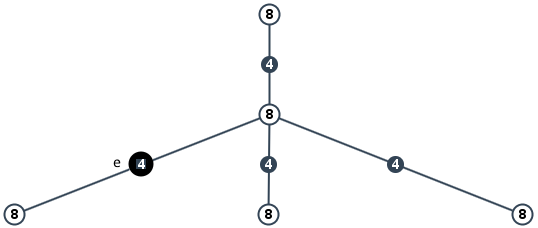
\includegraphics[width=0.7\textwidth]{bilder/abb1_NEU2.png}} 
		%		\hfill
		
		\subfigure[Eine Kante wurde auf Gewicht 1 geduziert, alle anderen Kanten haben weiterhin Gewicht 4. Alle Knoten benötigen trotzdem mindestens 8 Agenten.]{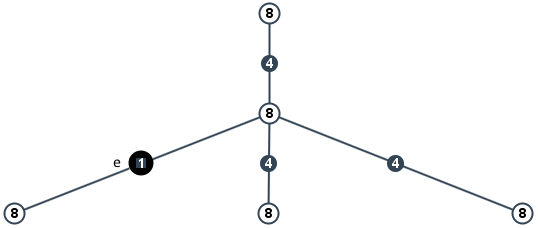
\includegraphics[width=0.7\textwidth]{bilder/abb2_NEU2.png}} 
		\captionsetup{width=0.9\textwidth}
		\caption{Beispiel, dass Verringerung auf einer Kante nicht zu einer Verringerung der notwendigen Agenten führen muss} 
		\label{abb_gegenbeispielMaxPotential}
	\end{figure} 
	
	Da das Potential in diesem Gegenbeispiel nicht angewendet werden kann, ist dies ein Widerspruch zur Annahme, dass man die Agentenanzahl auf einem beliebigen Baum mit beliebig großem Potential immer reduzieren kann.
\end{proof}

Trotzdem ist es möglich, einen Algorithmus anzugeben, der die Kante auswählt, welche die Agentenanzahl am meisten reduziert. Falls es keine solche Kante gibt, kann das Potential nicht angewendet werden und der Algorithmus gibt diese Information aus.


\subsubsection{Algorithmusidee}

	Um dieses Problem zu lösen, muss die in Kaptiel \ref{modifizierterAlgoChapter} benutzte Nachricht angepasst werden. Die Idee dieses Algorithmus ist - ähnlich wie beim Spezialfall $k = 1$ -  Protokoll zu führen. Damit lässt sich im Anschluss bestimmen, welche Kante am sinnvollsten reduziert werden muss.\\
	Jeder Knoten $x$ soll am Ende des Algorithmus folgende Informationen haben:
	\begin{itemize}
		\item $\mu(x)$: die normale Agentenanzahl (wird wie in Kapitel \ref{modifizierterAlgoChapter} ganz normal berechnet)
		\item $\hat{\mu}(x)$: die benötigte Anzahl an Agenten, die durch für diesen Knoten optimale Anwendung des Potentials erreicht werden kann
		\item $e_{1}, e_{2}$: die Kanten, auf die das Potential angewendet werden muss, um $\hat{\mu}(x)$ zu erreichen
	\end{itemize}
	Hat jeder Knoten am Ende der Berechnung diese Informationen, kann der Algorithmus mit einem Durchlauf durch alle Knoten das Minimum aller $\hat{\mu}$ ermitteln. Dies ist dann die kleinste Anzahl an Agenten, die durch das Potential erreicht werden kann. Da außerdem gespeichert ist, welche Kanten dafür reduziert werden müssen, kann man auf eine dieser Kanten das Potential anwenden, um die Agentenzahl entsprechend zu reduzieren. Wie in Theorem \ref{theorem_max2kanten} argumentiert, kommen immer nur maximal zwei Kanten pro Knoten in Frage.
	
	
	\subsubsection{Berechnung der Nachrichten}
	
	Um diese Informationen zu generieren, müssen die Nachrichten erweitert werden.
	Diese enthalten nun folgende Parameter:
	\begin{itemize}
		\item $\alpha$: die normal berechnete Nachricht (siehe Kapitel \ref{modifizierterAlgoChapter})
		\item $\beta$: modifizierte Nachricht, die durch das Potential am stärksten reduzierte Nachricht
		\item $e_{1} / e_{2}$: die Kanten, auf die das Potential angewendet worden ist
	\end{itemize}
	Es bleibt noch zu klären, wie die modifizierte Nachricht $\beta$ und die Kanten $e_{1}$ und $e_{2}$ berechnet werden.\\
	Bei jeder Berechnung einer neuen Nachricht kommen nur bis zu vier Möglichkeiten in Frage, wie das Potential angewendet werden kann, um die richtige modifizierte Nachricht zu generieren. Diese vier Möglichkeiten sind: $edge_{1}$, $edge_{2}$, $edge_{xy}$ (also die Kante, über die die Nachricht geschickt wird) und die Protokollierung von $l_{1}$ als größte Nachricht. Um nun herauszufinden, wie das Potential an dieser Stelle am effektivsten angewendet werden muss, werden alle vier Möglichkeiten nacheinander ausprobiert und dann entschieden, wo das Potential die größte Reduzierung zur Folge hatte. Der Fall mit dem größten Effekt wird in der neuen Nachricht gespeichert.
	\\
	\\
	Wir gehen alle Fälle durch, um die modifizierte Nachricht $\beta$ von Knoten $x$ nach $y$ zu berechnen:
	\begin{enumerate}
		\item berechnet $\beta$, indem das Potential auf die Kante zwischen x und y angewendet wird ($\beta = edge_{xy} - potential$)
		\item berechnet $\beta$, indem das Potential auf die größte Kante $edge_{1}$ angewendet wird ($\beta = edge_{1} - potential$) 
		\item berechnet $\beta$, indem das Potential auf die zweitgrößte Kante $edge_{2}$ angewendet wird ($\beta = edge_{2} - potential$)
		\item berechnet $\beta$, indem aus $l_{1}$ nicht die normale Nachricht $\alpha$, sondern die modifizierte Nachricht $\beta$ verwendet wird
	\end{enumerate}
	Der kleinste $\beta$-Wert aus diesen vier Fällen ist unsere modifizierte Nachricht $\beta$. Die Kanten, auf die das Potential angewendet wurde, wird als 3. Parameter $e_{1} / e_{2}$ in der Nachricht mit verschickt.\\
	Treten mehrere Fälle auf, die zu einen identischen $\beta$-Wert führen, so muss ein weiterer Test durchgeführt werden, ob es sich um die gleichen Kanten $e_{1} / e_{2}$ handelt. 
	\\
	\\
	Zu beachten ist noch, dass jede Kante zu jeder Zeit ein Kantengewicht $\omega \geq 1$ haben muss. Also wenn z.B. $edge_{1} - potential$ einen Wert $\beta < 1$ liefert, muss dieser Wert auf 1 gesetzt werden.
	\\
	\\
	Die Vorgehensweise ändert sich im Gegensatz zu dem Algorithmus aus Kapitel \ref{modifizierterAlgoChapter} nicht. Auch das $\alpha$ der Nachricht wird, wie im Algorithmus beschrieben, berechnet.
	
	
	\subsubsection{Berechnung der minimalen Agentenzahl}
	
	Um nun das $\hat{\mu}$ jedes Knotens zu berechnen, wird analog zur Berechnung der Nachricht vorgegangen. Der einzige Unterschied ist, dass es einen Fall weniger gibt: 
	\begin{enumerate}
		\item berechnet $\hat{\mu}$, indem das Potential auf die größte Kante $edge_{1}$ angewendet wird ($\hat{\mu} = edge_{1} - potential$) 
		\item berechnet $\hat{\mu}$, indem das Potential auf die zweitgrößte Kante $edge_{2}$ angewendet wird ($\hat{\mu} = edge_{2} - potential$)
		\item berechnet $\hat{\mu}$, indem aus $l_{1}$ nicht die normale Nachricht $\alpha$, sondern die modifizierte Nachricht $\beta$ verwendet wird
	\end{enumerate}
	Da wir keine Nachricht mehr verschicken müssen, sondern nur noch das $\hat{\mu}$ ausrechnen wollen, fällt der Fall, in dem die Kante $edge_{xy}$ reduzieren werden muss, weg.\\
	Nachdem der Algorithmus für jeden Knoten die drei Parameter ausgerechnet hat, besitzt jeder Knoten die Information, wie viele Agenten an diesem gebraucht werden, wenn das Potential nicht angewendet wird ($\mu$); wie viele Agenten benötigt werden, wenn das Potential angewendet wird $\hat{\mu}$; und auf welche Kanten das Potential angewendet werden muss, um diese Verbesserung zu erreichen (die Kanten, die zur Berechnung von $\hat{\mu}$ reduziert wurde).\\
	Durch einen linearen Durchlauf durch alle Knoten kann der Algorithmus das Minimum aller $\hat{\mu}$ berechnen und die dazugehörige(n) Kante(n) auswählen, auf die das Potential sinnvoll angewendet werden kann.
	\\
	\\
	Analog zur Nachrichtenberechnung muss jede Kante zu jedem Zeitpunkt der Berechnung ein Kantengewicht $\omega \geq 1$ haben. 
	
	
	\subsubsection{Laufzeit und Korrektheit}
	
	\begin{theorem}
		Die Berechnung aller Nachrichten und die Bestimmung der Kante, auf die das Potential angewendet werden sollte, ist in linearer Laufzeit möglich.
	\end{theorem}
	\begin{proof}
		Analog zu Theorem \ref{thm_laufzeit_modifikation} wird die Grundidee des Algorithmus nicht verändert. Jeder Knoten schickt zu all seinen Nachbarn je eine Nachricht. Die Anzahl der Nachrichten ändert sich durch die Modifikation nicht, sondern nur die Berechnung an sich.\\Die Berechnung der Nachricht kann auch hier in konstanter Zeit durchgeführt werden, da pro Nachricht nur maximal vier konstante Fälle berechnet werden müssen, und aus diesen das Minimum bestimmt werden muss.\\
		Auch die Berechnung der minimalen Agenten ist für jeden Knoten in konstanter Zeit möglich, wodurch der ganze Algorithmus eine Laufzeit von $O(n)$ hat.
	\end{proof}
	
	
	Um nun die Korrektheit des Algorithmus zu zeigen, muss man garantieren, dass jeder Knoten alle ausgehenden Nachrichten richtig berechnet. Wie beschrieben, enthält jede Nachricht drei Teilinformationen: $\alpha$, die normal berechnete Nachricht; $\beta$, die Nachricht, die man erhält, wenn im aktuellen Teilbaum das Potential optimal angewendet wurde; und $e_1/e_2$, die zwei Kanten, auf die das Potential angewendet werden muss, um die optimale Nachricht $\beta$ zu erhalten.
	\\
	\\
	Für die Korrektheit dieses Algorithmus ist nur $\beta$ interessant, da $\alpha$ die identische Nachricht aus Kapitel \ref{modifizierterAlgoChapter} ist, und die Kanten $e_1/e_2$ einfach aktualisiert werden können, wenn $\beta$ verändert wird. Daher können wir aus folgender Invariante schließen, dass der Algorithmus das Potential bis zum aktuellen Zeitpunkt richtig berechnet hat.
	
	\begin{theorem}
		Jeder Knoten im Baum berechnet korrekt, ob, und wenn ja, wo im aktuellen Teilbaum das gegebene Potential am effektivsten angewendet werden kann. Außerdem wird berechnet, wie groß die benötigte Agentenzahl nach Anwenden des Potentials für diesen Teilbaum ist.
	\end{theorem}
	\begin{proof}
		Um für die Korrektheit dieser Aussage zu argumentieren, muss man sich zwei Arten von Knoten anschauen: Blattknoten und innere Knoten im Baum.\\
		\\
		Zuerst betrachten wir die Blattknoten.\\
		Zu jedem Blatt führt genau eine Kante. Daher kann das Potential nur auf dieser einen Kante angewendet werden. Wenn die Nachricht nun von diesem Knoten berechnet wird, muss bei der Berechnung nur überprüft werden, ob sich die Nachricht verringert, wenn das Kantengewicht um das Potential reduziert wird. Dies ist immer der Fall, wenn das Kantengewicht $\omega > 1$ ist, da dadurch die Kante reduziert werden kann, und man daher für diesen Teilbaum weniger Agenten benötigt.
		\\
		\\
		Betrachten wir nun einen beliebigen Knoten $x$ innerhalb des Baumes.\\
		Wir gehen davon aus, dass bis zu diesem Zeitpunkt alle Nachrichten korrekt berechnet wurden. Dann muss der Knoten $x$ aus allen seinen angekommenen Nachrichten die neue Nachricht berechnen.\\
		Der Knoten $x$ hat die Information, wie viele Agenten die einzelnen Teilbäume brauchen, wenn das Potential nicht angewendet wird, (dies ist die normale Nachricht $\alpha$,) und, wie viele Agenten die einzelnen Teilbäume benötigen, wenn das Potential in diesen angewendet wurde (dies ist der $\beta$-Wert der einzelnen Nachrichten). Außerdem kennt der Knoten $x$ all seine inzidenten Kanten.\\
		Das einzige, was jetzt noch garantiert werden muss, ist, dass der Knoten $x$ alle Informationen aus den einzelnen Teilbäumen und aus seinen inzidenten Kanten richtig zusammensetzt, und somit eine Nachricht an einen Knoten $y$ berechnet, die für den gesamten Teilbaum gilt.\\
		\\
		Es sind nur drei Kanten bei der Berechnung interessant: Die Kante, über welche die Nachricht von $x$ nach $y$ geschickt wird, sowie die zwei größten Kanten $edge_1$ und $edge_2$, inzident zu $x$. Wenn eine andere Kante in diesem Teilbaum besser geeignet ist für das Potential, wurde sie schon in einer der Nachrichten an $x$ gespeichert. 
		\\
		\\
		Der Knoten $x$ muss daher nur testen, ob sich der $\beta$-Wert verbessert, wenn das Potential auf einer der drei Kanten angewendet, oder wenn der $\beta$-Wert von $l_{1}$ (also der größten angekommenen Nachricht) benutzt wird. Die Variante mit dem größten Einfluss ist der Wert für die neue Nachricht, und die entsprechende(n) Kante(n) werden in $e_1/e_2$ protokolliert. Genau diese Fallunterscheidung führt der Algorithmus aus, um die Nachricht zu berechnen.
		\\
		\\
		Die Berechnung von allen $\mu$-Werten erfolgt analog zu der Nachrichtenberechnung, so dass jeder Knoten die drei Parameter $\alpha$, $\beta$ und $e_1/e_2$ berechnet. \\
		Mit einem Durchlauf durch alle Knoten kann die größte Auswirkung des Potentials gefunden werden, sowie die zugehörigen Kanten, auf die das Potential angewendet werden kann.
		\\
		\\
		Falls es keine Möglichkeit gibt, das Potential anzuwenden, so gilt $\min \beta = \min \alpha$. Dies ist der Fall, wenn sich die minimale Anzahl an Agenten unabhängig von der Potentialanwendung nicht verändert.
	\end{proof}
	
	

\subsection{Potential verteilen mit $k > 1$}\label{kap_pot>1_verteilt}

Die nächste Erweiterung des Potentialproblems ist, Potentiale $k > 1$ zu betrachten, bei denen man das Potential auf verschiedene Kanten verteilen kann.\\
In Abbildung \ref{abb_gegenbeispielMaxPotential} haben wir bereits ein Beispiel gesehen, in dem es tatsächlich nötig sein kann, das Potential auf verschiedene Kanten zu verteilen. Dieses Beispiel soll im Folgenden erweitert werden.

\begin{theorem}\label{theorem_pot_auf_linear_vielen_kanten}
	Es gibt Bäume, bei denen das Potential auf linear viele Kanten verteilt werden muss.
\end{theorem}	
\begin{proof}
	Um dieses Theorem zu beweisen, reicht es aus, ein Beispiel anzugeben, bei dem das Potential tatsächlich auf linear viele Kanten verteilt werden muss. Solch ein Beispiel kann man in Abbildung \ref{abb_bsp_potverteilen} finden. Der Baum besteht aus einem Wurzelknoten, der $n$ viele Kindknoten hat. Alle $n$ Kanten haben das gleiche Kantengewicht $\omega = 5$.
	
		\begin{figure}[htb]
			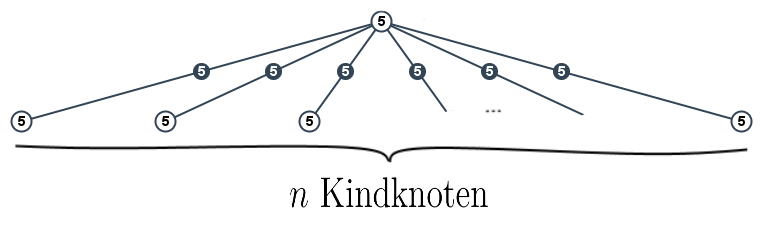
\includegraphics[width=0.75\textwidth]{bilder/abb_bsp_potverteilen.png} 
			\captionsetup{width=0.75\textwidth}
			\caption{Die Mindestanzahl an benötigten Kanten kann bei der Potentialverteilung eine Komplexität linear zur Knotenanzahl haben.}
			\label{abb_bsp_potverteilen}
		\end{figure}
		
	Um nun bei diesem Baum durch ein Potential $k$ die Agentenzahl verringern zu können, muss $k$ auf $n-2$ vielen Kanten angewendet werden, wobei $n$ die Anzahl der Kindknoten ist. Daraus folgt direkt, dass $k$ mindestens $n-2$ groß sein muss, damit wir das Potential überhaupt auf den Baum aus unserem Beispiel anwenden können. Bei einem geringeren Potential kann man keine Verbesserung erzielen.
	\\
	\\
	Bleibt noch zu klären, warum das Potential auf $n-2$ Kanten angewendet werden muss.
	\\
	Wie in Kapitel \ref{modifizierterAlgoChapter} beschrieben, kann eine Nachricht $\lambda_{x}$ aus drei Fällen bestehen:
	\begin{enumerate}[label=\alph*)]
		\item aus den zwei größten Nachrichten: $\lambda_{x} = edge_{1} + edge_{2}$
		\item aus der Kante, über welche die Nachricht geschickt wird: $\lambda_{x} = edge_{xy}$
		\item aus der größten Nachricht: $\lambda_{x} = l_{1}$
	\end{enumerate}	
	Allerdings ist nur der Fall $\lambda_{x} = edge_{1} + edge_{2}$ interessant, da sowohl die Kante $edge_{xy}$ eindeutig ist als auch die größte angekommene Nachricht.
	\\
	\\
	Wenn man nun eine einzige beliebige Kante reduziert, wird diese Reduzierung keinen Effekt haben, da diese Kante in der Berechnung $\lambda_{x} = edge_{1} + edge_{2}$ durch eine andere, gleich große Kante, ersetzt wird. Um also das Potential anwenden zu können, so dass tatsächlich die Agentenzahl an einem Knoten $x$ reduziert wird, muss man so lange eine Kante $e$ reduzieren, für die gilt: $\omega(e) = \max_{i} \omega(i)$ für alle zu $y$ inzidenten Kanten $i$, bis gilt $edge_{1} > edge_{2} \geq \dots \geq edge_{deg(y)-1}$
	\\
	Sobald diese Bedingung gilt, können die durch das Potential reduzierten Kanten nicht mehr ausgetauscht werden, da es keine Kante mehr gibt, die groß genug wäre. Die Berechnung $\lambda_{x} = edge_{1} + edge_{2}$ ist daher eindeutig, und es konnte durch die Potentialanwendung eine Verringerung der Agentenzahl an Knoten $x$ erreicht werden. 
	\\
	\\
	Dafür müssen genau $n-2$ Kanten reduziert werden, da man in dem Beispiel alle Kanten reduzieren muss, außer die Kante $e = \{xy\}$, über die die Nachricht geschickt wird, und die Kante $edge_{1}$. Alle $n$ Kanten, abzüglich dieser beiden Kanten, ergibt $n-2$ Kanten.
	\\
	\\
	Die Idee dieses Beweises lässt sich auch aus Theorem \ref{theorem_max2kanten} herleiten, bei in dem eine ähnliche Eigenschaft ausgenutzt wurde.
	
\end{proof}


Bei den Potentialproblemen $k = 1$ (Kapitel \ref{kap_pot=1})und $k \geq 1$ auf einer Kante (Kapitel \ref{kap_pot>=1}) musste man für jede Nachrichtenberechnung nur konstant viele Kanten testen, und es war daher möglich, einen Algorithmus zu entwerfen, der ohne Laufzeitverschlechterung die jeweilige Kante bestimmen konnte.
\\
Diese praktische Eigenschaft scheint bei der Verteilung des Potentials nicht mehr gegeben. Da es nach Theorem \ref{theorem_pot_auf_linear_vielen_kanten} sein kann, dass man das Potential auf fast alle Kanten verteilen muss, kann es passieren, dass alle bisher betrachteten Kanten in der Nachricht gespeichert werden und bei jeder neuen Nachricht mit überprüft werden müssen. In den Varianten, bei denen das Potential nur auf einer Kante angewendet werden darf, war diese Anzahl auf zwei beschränkt (siehe Theorem \ref{theorem_max2kanten}).
\\
\\
Es war daher nicht möglich, im Rahmen dieser Bachelorarbeit eine Algorithmusidee zu entwickeln, um das Potentialproblem $k > 1$, bei dem das Potential auf mehrere Kanten verteilt werden kann, effizient zu lösen. Naiv würde man das Problem lösen, indem man alle möglichen Kantenkombinationen, wie das Potential verteilt werden kann, ausrechnen würde, und dann die Kombination mit der kleinsten Agentenanzahl auswählt.


%	\begin{figure}[htb]
%		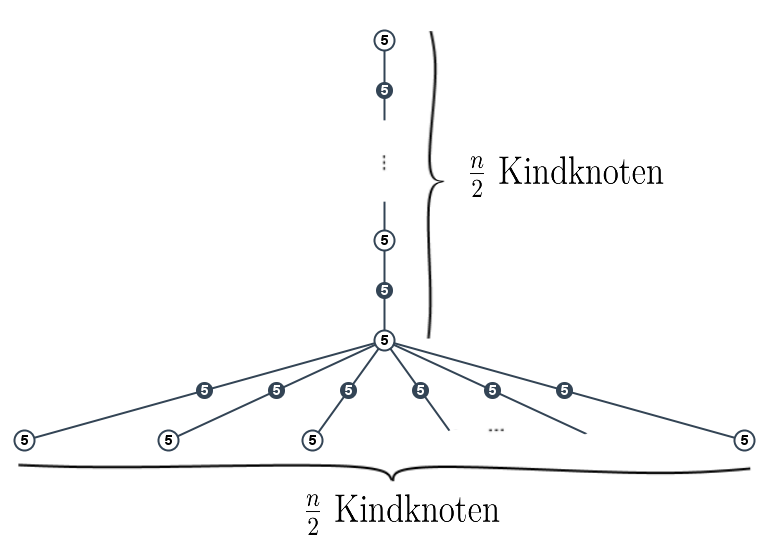
\includegraphics[width=0.65\textwidth]{bilder/abb_bsp_potverteilen_quadratisch.png} 
%		\captionsetup{width=0.65\textwidth}
%		\caption{Die Mindestanzahl an benötigten Kanten kann bei der Potentialverteilung kann eine Komplexität linear zur Knotenanzahl haben.}
%		\label{abb_bsp_potverteilen_quadratisch}
%	\end{figure}
